\documentclass[notitlepage]{article}

\usepackage{epstopdf}
\usepackage{bibunits}
\usepackage{comment}
\usepackage{graphicx}
\usepackage{amsmath}
\usepackage{datetime}
\usepackage{numprint}
\usepackage{palatino}
\usepackage{url}
\usepackage{footmisc}
\usepackage{endnotes}
\usepackage{listings}
\usepackage[colorlinks=true, urlcolor=blue, linkcolor=red]{hyperref}

\setcounter{secnumdepth}{3}
\begin{document}

\nplpadding{2}
\newdateformat{isodate}{
    \THEYEAR -\numprint{\THEMONTH}-\numprint{\THEDAY}}

\title{Project Freedom Extended Report}
\author{Gabriel Aldous\\MAS4115}
\date{\isodate\today}

\maketitle

\tableofcontents

\newpage
\section{Executive Summary}

\subsection{Project Overview}

Project Freedom is a easy to use CLI program that
users can interact with in order to perform their own experiments
with the Fast Fourier Transform and related operations on both images and audio files.
Basic filtering operations are supported for images and audio, and
there are numerous ways to visualize how the files have changed
and preview those changes. Additionally, the application supports
easy modification of the file system, and the classes employed
to perform these image modifications can easily be repurposed by
other programmers to add additional functionalities.
\\\\
In addition to the basic manipulations, there is an implemented
advanced 'hybridization' technique for both audio and image files.
Image files can be 'hybridized' so that the image appears to be one
thing up close, and another when viewed from far away, while audio
files can be modified to make it appear that one sound is being heard
within a different environment.
\\\\
This project is implemented in Python, and supports building on
Python versions 3.9-3.12 (though it was only tested on version 3.12).
It relies on Numpy, Matplotlib, Scipy, and PyGame, and instructions for
setting up and running the program are available in the README file.
To view the results of various operations performed by Project Freedom,
see the github repository.
\\\\
\subsection{Mathematical Principles}

The fundamental operation which this program seeks to
foster a greater understanding of is called the Fourier
Transform, or more specifically the Fast Fourier Transform (FFT).
This technique is often used in signal processing applications,
as is the case in this project. The FFT is utilized to turn some
signal data (such as an image or an audio file) into a different domain
called the frequency domain. Simply speaking, the FFT takes the input and
restructures it so that information about which frequencies are more prevalent
is easily accessible.
\\\\
In the context of the custom hybridizations, audio hybridization is performed using
a convolution, while image hybridization is performed by filtering the high detail portions
of one image (the edges \& lines) and overlaying it on the low detail portion of another
image (the general colors \& shapes). This results in an image which can trick human perception
and appear differently from different viewing distances.
\\\\
The FFT has applications in many areas, notably in image compression formats
like JPEG and MP3, filtering operations, wireless communication, and much more.
For more details about how the FFT works, and the linear algebra supporting it,
view the mathematics explanation section of this document.

\section{Motivation}

When considering the potential avenues of exploration for Project Freedom, there were
2 main paths which I considered. The first identifying malware files utilizing neural networks,
was interesting but I didn't feel comfortable installing thousands of files of malware onto my
laptop, even within a VM environment. That left this option of exploration, which was appealing
due to how it ties into my current coursework (Fourier Analysis) and future coursework
(a CS technical elective about 3D Audio). Additionally, this was motivated by my Fourier Analysis
course not covering the Fast Fourier Transform due to time constraints, so this became a nice
way to apply linear algebra and the skills I learned in that course to a practical application.

\section{Technical Report}

This portion of the report shall primarily cover how to setup the repository,
and show off various results from the program execution.

\subsection{Installation \& Use}
To run Project Freedom yourself, you can install the program with the following commands
from within a linux terminal.
\begin{lstlisting}
    git clone https://github.com/Sn00pyW00dst0ck/project_freedom.git
    cd project_freedom
    pip3 install -r requirements.txt
\end{lstlisting}
Note: on some systems 'pip3' may need to be replaced by 'pip'.
\\\\
With the project installed, the program can be run by executing the
following command from within the terminal in the BASE directory for
the project (if you run the executable from anywhere else, then the
program may attempt to read files from locations which do not exist,
and may crash):
\begin{lstlisting}
    python3 ./src/main.py
\end{lstlisting}
Note: on some systems 'python3' may need to be replaced by 'python'.
\\\\
When the project is executed, the user will be presented with a series of
menu options to determine which actions they wish to preform. The menu systems
are designed to walk the user through the operations which can be performed.

\subsection{Program Execution Results}

While I will briefly discuss some program execution results here, it is worth
noting that audio files cannot be adequately represented within a PDF document.
For this reason, I highly recommend viewing the 'samples' folder within the GitHub
repository to listen to the execution results which I will be discussing, particularly
in regards to audio.

\subsection{Audio Outputs}

The audio outputs created by Project Freedom mostly need to be heard to be
believed, though there are some graphs which can be shown here. Keep in mind,
the visualizations for each chart are different, particularly in the
axis scales, in other words, not all charts are drawn to scale! That said,
I highly recommend viewing the GitHub repository for this portion of the
report.
\\\\
We can view the effect of applying filters to the audio frequencies. For instance,
take the below audio waveform from the sapce\_oddity.wav file (which is a snippet of
David Bowie's song Space Oddity):
\\
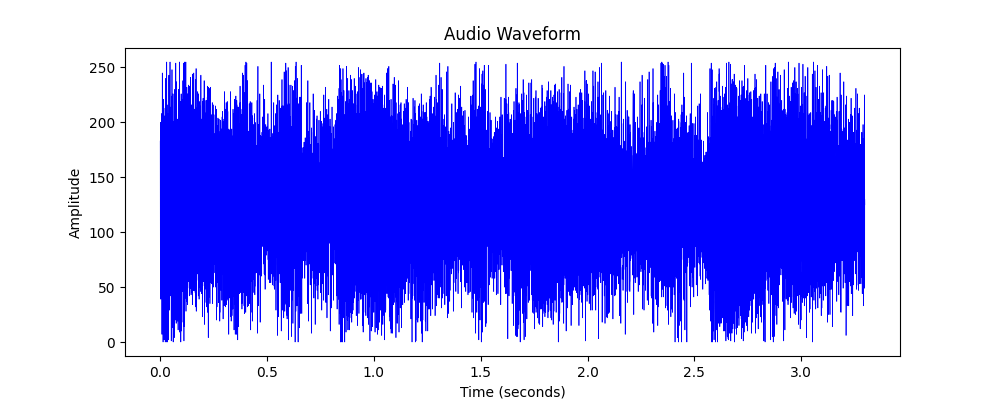
\includegraphics[width=4.75in]{../samples/audio/space_oddity_waveform.png}
\\
We can view the fourier transform of this waveform below:
\\
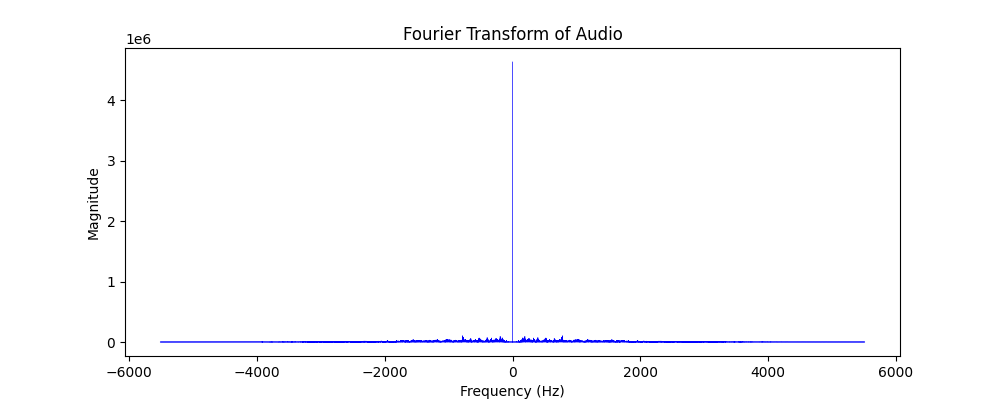
\includegraphics[width=4.75in]{../samples/audio/space_oddity_fourier_transform.png}

Now, we can filter out the low frequency audio by applying a low-pass filter. Observe
the effects on each graph:
\\
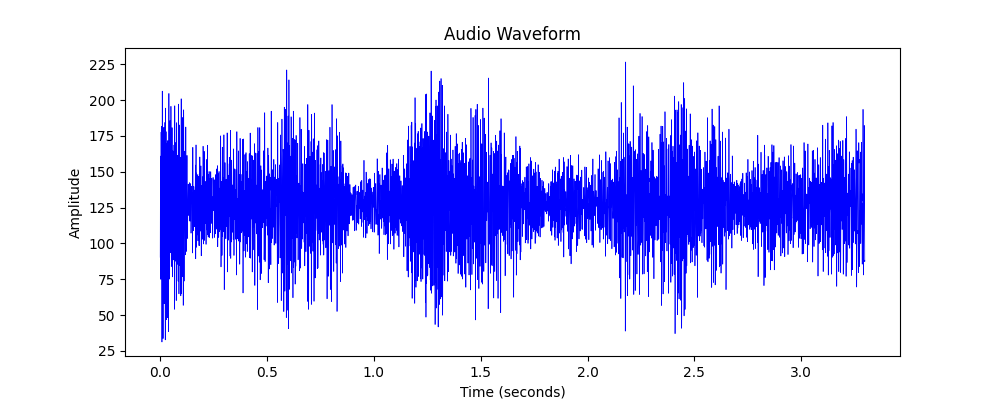
\includegraphics[width=4.75in]{../samples/audio/space_oddity_low400_waveform.png}
\\
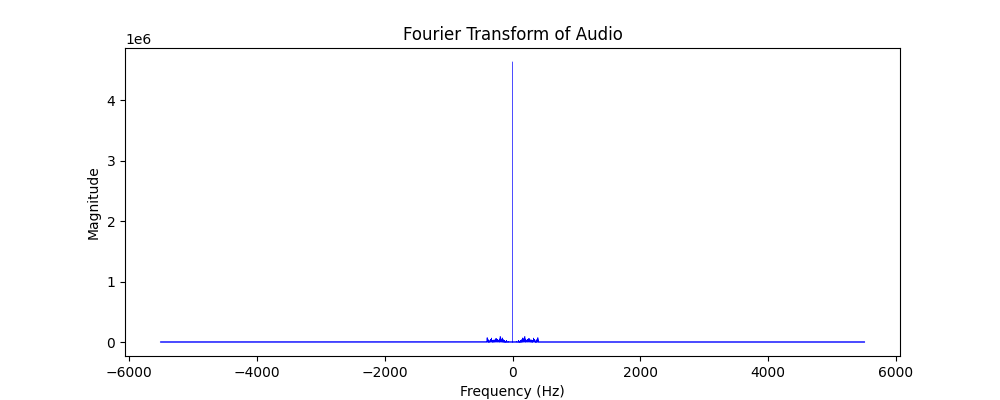
\includegraphics[width=4.75in]{../samples/audio/space_oddity_low400_fourier_transform.png}
\\
We can tell from the waveform that an operation was applied to the original audio, but it isn't
possible to make an accurate guess at what the operation was. Observing the Fourier Transform of the
audio though, it is clear to see that the frequencies past 400Hz were removed. A similar
result for the same audio file can be seen when applying a high-pass filter (which keeps the
higher frequencies).
\\
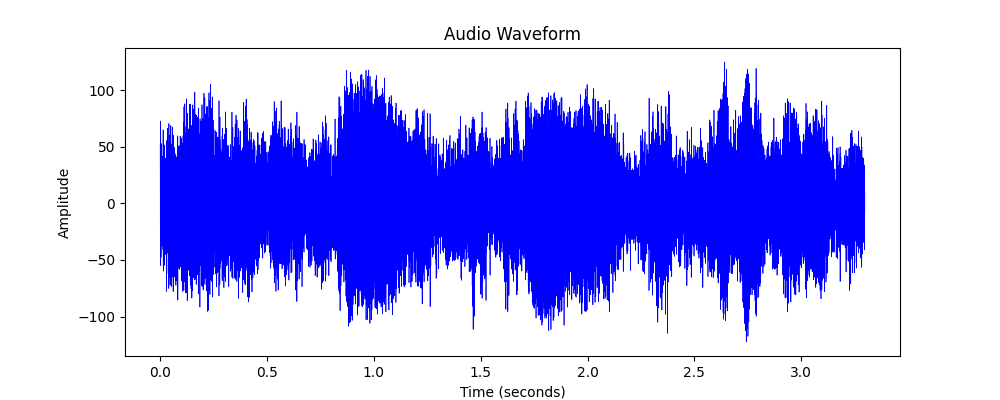
\includegraphics[width=4.75in]{../samples/audio/space_oddity_high750_waveform.png}
\\
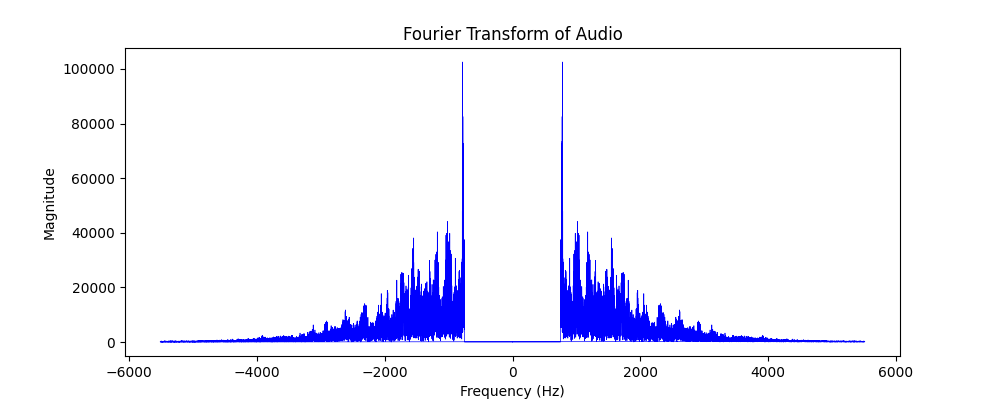
\includegraphics[width=4.75in]{../samples/audio/space_oddity_high750_fourier_transform.png}
\\
Additionally, when listening to the audio files, it is clear to tell that one is clearly
much higher pitched than the original file (though you may need to turn the volume up high to
hear it).
\\\\
Beyond filtering data, the other main audio process that Project Freedom supports is
convoluting audio files together. In this context, convoluting two audio files together
can be thought of as taking a weighted average of the sounds, so that the first sound appears
to be played within the environment of the second sound. This too, is done in the frequency space. We turn our
attention to a new audio file, one of a dog barking.
\\
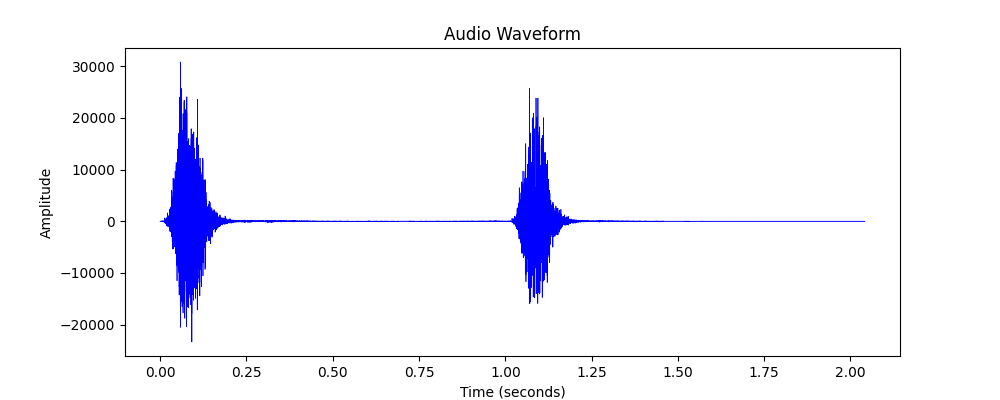
\includegraphics[width=4.75in]{../samples/audio/dog_bark_dry_waveform.png}
\\
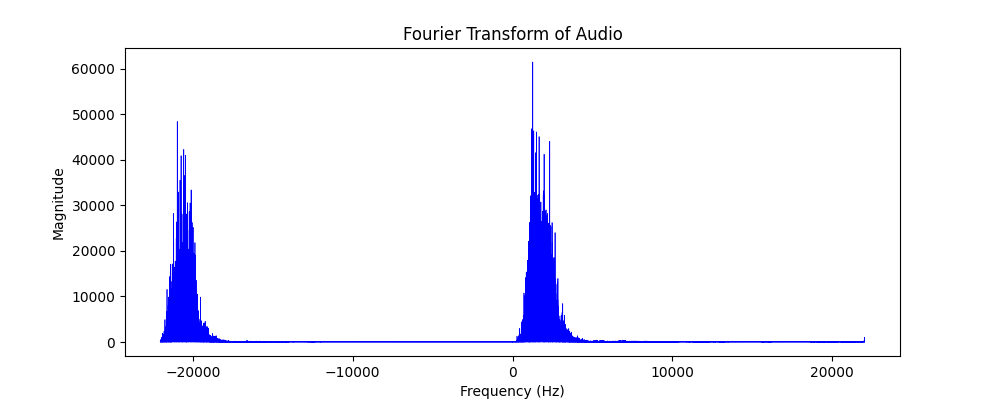
\includegraphics[width=4.75in]{../samples/audio/dog_bark_dry_fourier_transform.png}
\\
Below I will show two different convolutions of the dog barking sound, one in a cave
environment with lots of echo, and another in a forest environment with considerably
less echo.
\\\\
The cave:
\\
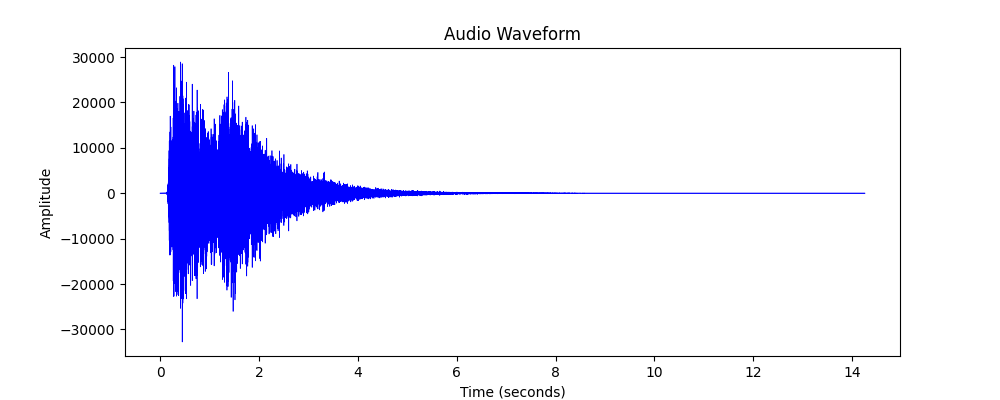
\includegraphics[width=4.75in]{../samples/audio/dog_bark_dry_convolve_cave_waveform.png}
\\
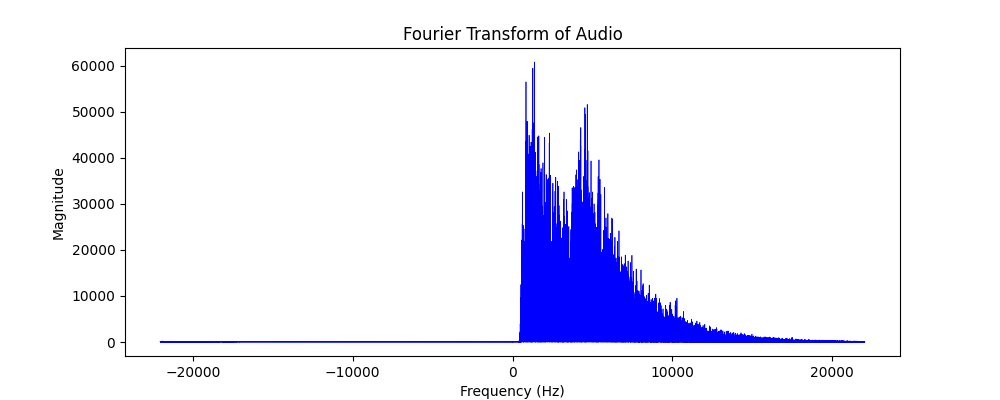
\includegraphics[width=4.75in]{../samples/audio/dog_bark_dry_convolve_cave_fourier_transform.png}
\\
The forest:
\\
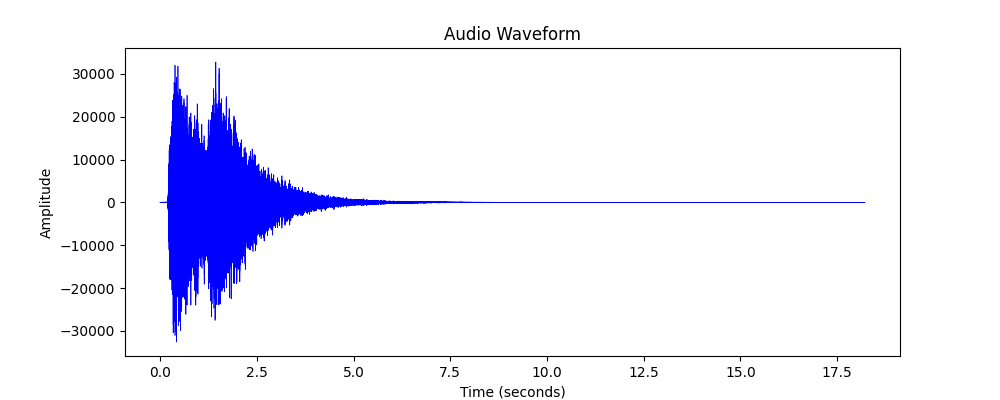
\includegraphics[width=4.75in]{../samples/audio/dog_bark_dry_convolve_forest_waveform.png}
\\
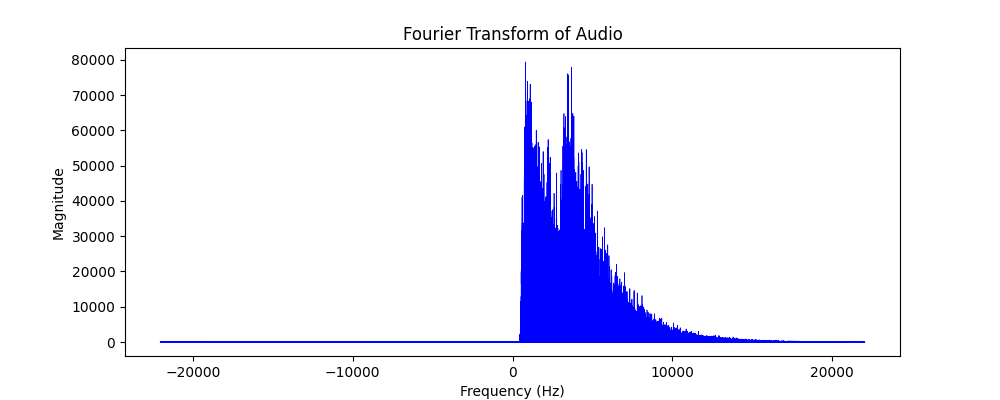
\includegraphics[width=4.75in]{../samples/audio/dog_bark_dry_convolve_forest_fourier_transform.png}
\\
On the surface, these output results seem very similar, but when noticing
the time axis, it is clear to see that the cave audio will play for
much longer than that of the forest (which makes sense when considering the
echo effect of a cave).

\subsection{Image Outputs}

The image outputs created by Project Freedom are much easier to visualize,
though how the operations are being applied becomes less obvious due to the
2 dimensional nature of images. Essentially, the images can be thought of as
a 'signal' in 2d space in a similar way to how we could visualize audio as a
1d signal (only instead of using the time dimension, we are using the x and y
dimensions).
\\
Let's consider the first image, one of Albert Einstein in black and white.
\\
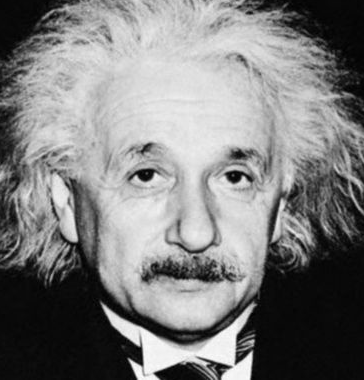
\includegraphics[width=4.75in]{../assets/images/einstein.png}
\\
It's fourier transform is represented by three channels, the first for red, the
second for green, and the third for blue. Since this is a black and white image,
they will all be the same, but in RGB images they would be different. The fourier transform
is shown below:
\\
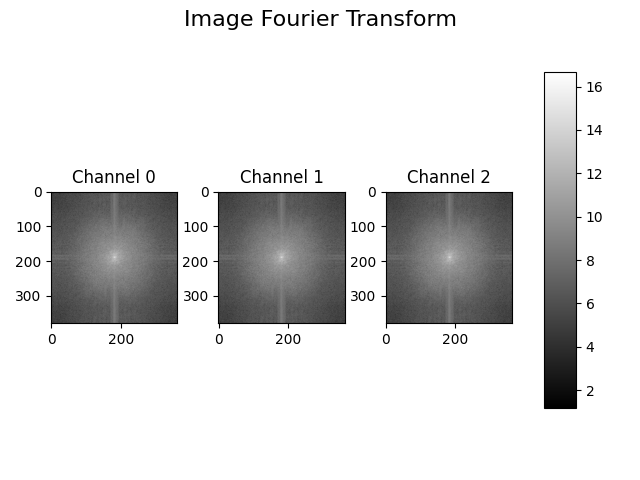
\includegraphics[width=4.75in]{../samples/images/einstein_fourier_transform.png}
\\
Just as with audio files, we can apply filtering operations to this (and other) images.
The high and low pass filters work the similarly to before, only now there is more nuance to
their application since we are in a 2d setting. Let's look at the low pass filter output
before explaining what is occurring:
\\
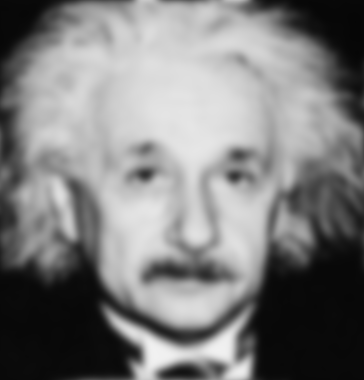
\includegraphics[width=4.75in]{../samples/images/einstein_low15.png}
\\
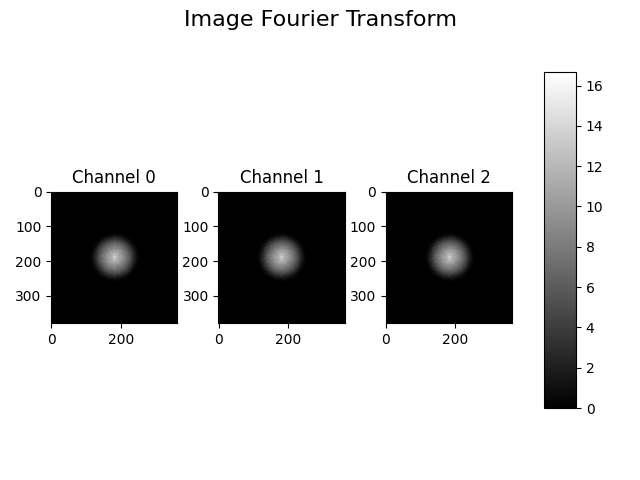
\includegraphics[width=4.75in]{../samples/images/einstein_low15_fourier_transform.png}
\\
It's pretty easy to tell that the image seems blurrier than the original one after
applying the low pass filter. Furthermore, inspection of the Fourier Transform
shows that only the frequencies corresponding to the 'center' of the frequency space
are being shown. Clearly, the center frequencies correlate to the low frequencies, and
as you move outwards in a circle the frequencies increase. This makes sense for 2d, as you
can move in both dimensions (x and y) at different rates, so a circle should appear. This is
further supported by the analysis of the low pass filter in the audio case, as a similar thing
appeared with the center portion of the frequency graph staying while the outer region was removed.
\\
Also, it's worth noting that in this implementation of filtering, we can no longer specify a single
frequency value to cutoff at. Instead, a kernel (in this case the Guassian kernel) is used to perform
the filtering, and a parameter called sigma is used to control how many frequencies are kept and removed.
Within this document, all sigma values used for filters are 15 unless otherwise noted.
\\\\
We can also inspect the high pass filter, which shows a similar trend (though much less pronounced).
\\
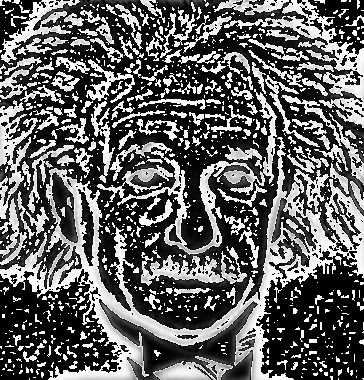
\includegraphics[width=4.75in]{../samples/images/einstein_high15.png}
\\
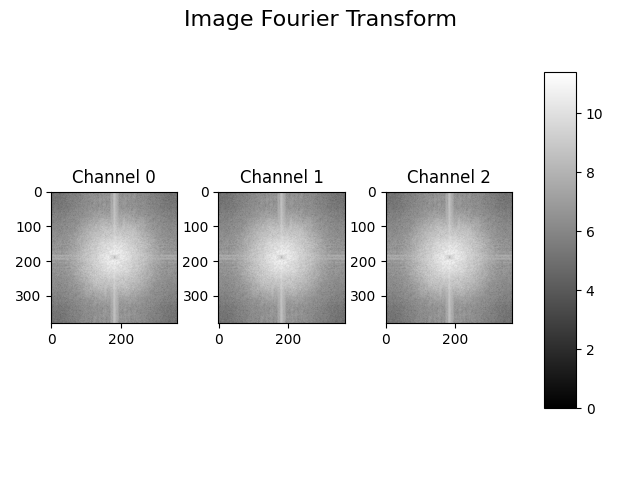
\includegraphics[width=4.75in]{../samples/images/einstein_high15_fourier_transform.png}
\\
Here, we can easily tell that all the sharp features (the lines and edges of the image),
have been emphasized. Furthermore, it is possible to see a slight darkening in the
center of the fourier transform of the new image.
\\\\
The observations from the high and low pass filters can tell us something interesting about
the frequency space of images. The outside (or high) frequencies correspond to the sharp
regions of the image (the lines and edges), while the center (or low) frequencies correspond
to large regions of color. We can exploit this observation in some neat ways, one of which is
outlined below.
\\\\
We can 'hybridize' images, in other words, we can combine one image with another sufficiently similar
image to create an image which appears to be two different things when viewed from up close or far away.
This is best done by providing an example, so let's take a look at merging our image of Einstein from
before with one of Marilyn Monroe (found in the assets folder). The combination of the two images looks like this:
\\
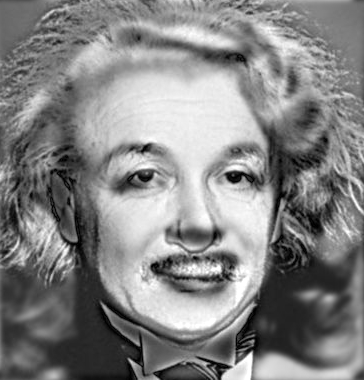
\includegraphics[width=4.75in]{../samples/images/einstein_monroe.png}
\\
If observed near the screen, the fine lines and details from the image of Albert Einstein dominate
the image and our brain perceives the image of Albert Einstein. However, stand sufficiently far away
(about 5-10 feet away) and the fine details of the Einstein image fade away and the portions taken from
the image of Marilyn Monroe take over, making us see her instead.
In this case, the sigma values used are 23 for the Einstein image (which gets high passed), and 14 for the image
of Marilyn (which gets low passed). Obviously, the resulting illusion effectiveness is highly dependent on how well
the sigma values are chosen, and how well the edges of the images align with each other.
\\\\
A logical question when seeing this technique is to ask "What about colored images?". Well, because of the properties of the
Fourier Transform, it is possible to apply this technique to them as well by applying the same operation to each channel individually.
Let's try this, by taking those same images of Einstein and Monroe and putting them through an AI image color generator, and then reapplying
our method.
\\
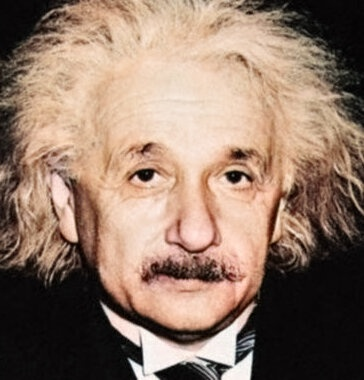
\includegraphics[width=4.75in]{../assets/images/rgb_einstein.png}
\\
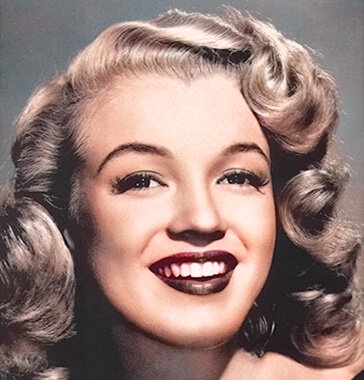
\includegraphics[width=4.75in]{../assets/images/rgb_monroe.png}
\\
Merging the two yeilds this result:
\\
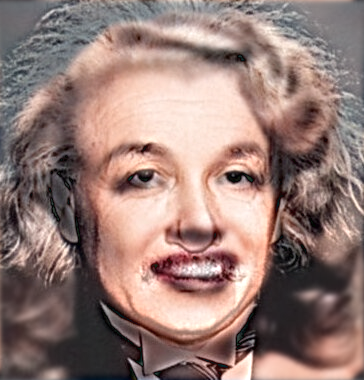
\includegraphics[width=4.75in]{../samples/images/rgb_einstein_monroe.png}
\\
We can see that the illusion still somewhat holds, but is clearly no longer so great. In particular,
the color data breaks the illusion when viewing the image from up close (particularly where the mouth
and hair are concerned). This highlights one major issue with this approach (at least when performed on colored images),
if the images need to be sufficiently similar to be hybridized, then is it worth the effort in the first place.

\section{Mathematical Explanation}

\subsection{Explanation of Fourier Transform and Fast Fourier Transform}

I want to make clear up front that the Fourier Transform will not be adequately covered
within this single report. The topic is extremely nuanced and the full applications of it
are still actively being researched. That said, I will attempt to provide a very brief explanation
of why the Fourier Transform works, and what the Fast Fourier Transform is doing.
\\\\
As previously stated, the main idea of the Fourier Transform is that we can
turn signal data into what is called the 'frequency domain'. But why exactly is
this called the frequency domain? Well, what the Fourier Transform does (in EXTREMELY
simplified terms) is transforms
the signal into an infinitely long series of sine and cosine functions (multiplied
by some constants). The idea is that as we add more and more sine and cosines onto
this sequence, we can get closer and closer to the original signal (though in many cases we
don't explicitly write the sines and cosines, instead using Euler's number and complex
exponents to represent them). Taking this idea
to infinity, we can match the original signal exactly.
\\\\
Of course, it is impractical for a computer to take this idea to infinity (we would
run out of memory, time, and energy to perform the computations), so the solution is
to stop the approximation once the sequence gets sufficiently close to the original signal.
This is known as a Discrete Fourier Transform (DFT). The DFT can be represented by this formula (\href{https://ccrma.stanford.edu/~jos/st/Matrix_Formulation_DFT.html}{source}):
\\
\begin{align*}
    X[k]=\sum_{n=0}^{N-1} x[n] * e^{-i\frac{2\pi}{N}kn}
\end{align*}
However, storing the sequence in this manner isn't very efficient. Instead,
the DFT is often represented in terms of matrices and vectors. In particular:
\begin{align*}
    X = F * x
\end{align*}
Where X is the DFT coefficients, F is the DFT matrix, and x is the input sequence (as a column vector).
The DFT matrix is simply an NxN matrix defined as below:
\begin{align*}
    A = \frac{1}{\sqrt{N}}\begin{bmatrix}
                              1      & 1            & 1               & \dots  & 1                   \\
                              1      & \omega       & \omega^2        & \dots  & \omega^{N-1}        \\
                              1      & \omega^2     & \omega^3        & \dots  & \omega^{2(N-1)}     \\
                              \vdots & \vdots       & \vdots          & \ddots & \vdots              \\
                              a_{K1} & \omega^{N-1} & \omega^{2(N-1)} & \dots  & \omega^{(N-1)(N-1)}
                          \end{bmatrix}
\end{align*}
Here, $\omega = e^{\frac{-2\pi{i}}{N}}$ to save space on the page, and the scaling term out front is
necessary to satisfy a crucial property of the Fourier Transform (known as \href{https://en.wikipedia.org/wiki/Parseval%27s_theorem}{Parseval's Theorem}).
Also, its important to know that when undoing the transformation, all the exponents simply swap their sign
from positive to negative and vice versa.
\\\\
The DFT matrix has some other interesting properties as well. It is a linear transformation, so applying the
Fourier Transform becomes a matrix multiplication, and inverting the transform becomes another matrix multiplication.
Also, while its eigenvalues (and multiplicities) are well known to be +1, -1, +i, and -i (\href{https://users.metu.edu.tr/ccandan/pub_dir/Eig_Structure_DFT_IEEE_SPM_Column_March2011.pdf}{source}), its eigenvectors are extremely complicated.
\\\\
Unfortunately, creating this matrix in a simple manner would be a quadratic time algorithm, which
is not effecient enough for many applications. Fortunately, there exists numerous
algorithms which can perform this construction in O(nlog(n)) time (collectively called the Fast Fourier Transform).
The most famous of these algorithms
uses a divide and conquer approach and exploits some properties of the DFT (which can be further
read about \href{https://vanhunteradams.com/FFT/FFT.html#The-Cooley-Tukey-FFT}{here}) to recombine
the small DFTs into the desired size. This approach is called the Cooley-Turkey algorithm, and has
been independently discovered a few time according to \href{https://faculty.washington.edu/seattle/physics541/%202010-Fourier-transforms/history-3.pdf}{this source}.

\subsection{Code Implementation}

Within the source code of Project Freedom, the implementation of the FFT
is offloaded to Numpy and Scipy libraries. The reasoning for this is two-fold.
Although the Cooley-Turkey algorithms isn't too complicated to implement,
these libraries are widely tested and will provide accurate results. Furthermore,
these libraries will provide a more robust implementation than one which has been hand coded
(both in terms of speed and versatility).
\\\\
To see a sample of how FFT is used within the Python code, we examine the
high\_pass\_filter method of the Audio\_Processor class:
\begin{lstlisting}
    def high_pass_filter(self, cutoff_frequency):
    """
    Apply a high pass filter to the loaded audio
    effectively isolating the high frequencies only.

    Args:
        cutoff_frequency (int): 
            The frequency at which to apply the filter.
    """
    if self.audio_data.ndim == 1:
        fft_audio = fft(self.audio_data)
        # Get the frequencies corresponding to each point in the FFT
        frequencies = np.fft.fftfreq(len(fft_audio), d=1.0/self.sample_rate)
        # Create a mask for frequencies above the cutoff
        filter_mask = np.abs(frequencies) >= cutoff_frequency
        # Apply the mask to the FFT
        filtered_fft = fft_audio * filter_mask
        self.audio_data = ifft(filtered_fft).real
        return
    
    for channel in range(self.audio_data.shape[1]):
        # Apply FFT to the audio signal
        fft_audio = fft(self.audio_data)

        # Get the frequencies corresponding to each point in the FFT
        frequencies = np.fft.fftfreq(len(fft_audio), d=1.0/self.sample_rate)

        # Create a mask for frequencies above the cutoff
        filter_mask = np.abs(frequencies) >= cutoff_frequency

        # Apply the mask to the FFT
        filtered_fft = fft_audio * filter_mask

        # Apply Inverse FFT to obtain the filtered audio signal
        self.audio_data[:, channel] = ifft(filtered_fft).real
\end{lstlisting}

This method has been chosen for examination as it is a typical use case for FFT within
the project. The program determines if the FFT will need to be used one time, or multiple
times based on how many channels of data are present (mono vs stereo). Then, the FFT
operation is utilized to convert a channel from the normal space to the 'frequency space'
(represented as fft\_audio). Further processing is utilized to get the individual frequencies
from this, which can create a mask to filter out certain frequencies which are unwanted.
The filter is applied with element wise multiplication, and then the inverst FFT is utilized
to restore the audio to a format which can be played.

\section{Lessons Learned}

Implementing Project Freedom has re-inforced the concepts which I learned within Fourier Analysis,
while also allowing me to further apply those skills in a practical setting. Meanwhile, writing
this extended report has alllowed me to further cement some linear algebra topics and solidify
my understanding of the Fourier Transform. This will prove invaluable to me in future coursework.
\\\\
Beyond that, I tackled some interesting programming issues during the creation of this repository
which have given me practice in setting up a proper Python development setting and solving interesting
program organization challenges. This practice could prove valuable in the future, whether in grad
school or a industry setting.

\end{document}